Figure~\ref{fig:next-capacity} compares model capacity, energy-matched
ranking error, and energy independence for 19 NEXT neural configurations.
The complete results are listed in Table~\ref{tab:next-classification}.

\begin{figure}[!htb]
\centering
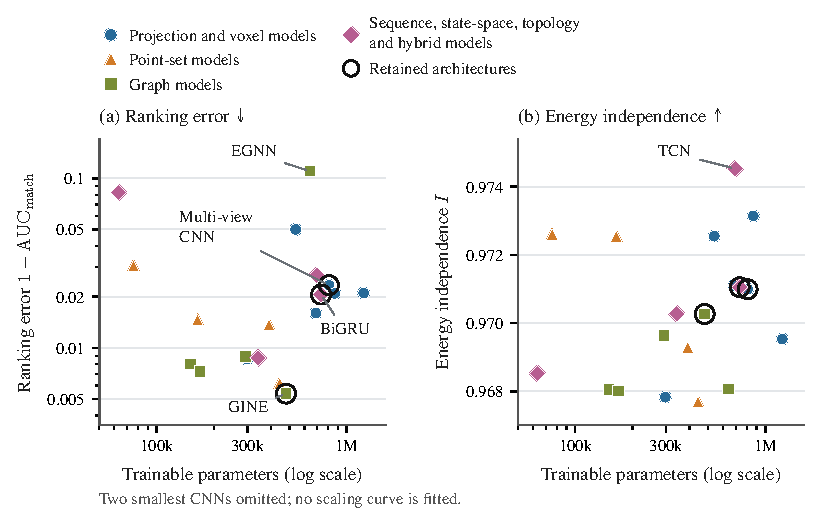
\includegraphics[width=\linewidth]{wing_contribution/figures/next_capacity_scores.pdf}
\caption{NEXT capacity comparison for 19 neural configurations on 116,549
test events (the shared 5 keV plus overflow protocol), excluding Two-conv CNN and Energy-skip CNN.
(a) Weighted pairwise ranking error $1-\mathrm{AUC}_{\mathrm{match}}$.
(b) Energy independence $I$. Parameter count and ranking error use log
scales; $I$ uses a linear scale. Colors and shapes identify four model
groups; black rings mark the three retained architectures with campaign
results. Earlier exploratory runs are excluded. The full inventory is in Table~\ref{tab:next-classification}.
No scaling curve is fitted.}
\label{fig:next-capacity}
\end{figure}


The shared classic-model reevaluation separates energy-matched ranking
from within-class score stability. The matched-AUC leaders among the available
retained-campaign classic models remain unchanged, while the independence values on EXO-200 and SuperNEMO are lower
under the finer common grid. The MJD and EXO-200 reevaluation excludes energies outside 0--3000 keV
without changing inclusive AUC. The reevaluated Transformers retain the
same matched-AUC leaders, while EXO-200 region--RoPE leaves the Transformer
Pareto set after its independence score decreases under the fixed grid.
These single-run comparisons describe the retained test populations and do
not establish statistical significance or performance under distribution shift.
